% -*- coding: utf-8 -*-
\chapter{Evolución y costes}
\thispagestyle{fancy}
%%\setcounter{page}{79}

\drop{E}{n} el presente capítulo se describirán las diferentes fases empleadas
en el desarrollo de \emph{FreeStation}, especificando los hitos característicos
de cada una, y aportando datos relacionados con la complejidad y el coste temporal de
cada una.

Igualmente se aportará información del rendimiento (profiling) del sistema en
diferentes situaciones, así como algunas comparativas con aplicaciones
demostrativas que no han sido desarrolladas utilizando \emph{FreeStation}.

\section{\uppercase{Fases e iteraciones}}

En este apartado se describe la aplicación del método ha conllevado una serie de
prácticas descritas por la XP para llegar a la solución.

Las primeras fases tenían como objetivo maximizar el valor del software
desarrollado como prototipo y pruebas de concepto iniciales para siguientes
iteraciones. Según los resultados producidos por iteración se han
retroalimentado las siguientes iteraciones. De esta forma, la valoración de 
costes y riesgos por cada iteración ha podido evaluarse según las tareas
completas y las planificadas por completar.

A continuación se describen las tareas realizadas y planificadas por fase.

\subsection{Fase 1 - Implementación prototipo}

En la primera fase se desarrollo una versión inicial como prototipo de cliente y
servidor usando sockets en Python. La implementación tiene una duración
aproximada de semana y media, donde se implementa una clase servidor que es 
iniciada como primera instancia, siendo los
parámetros por defecto el puerto y nodo donde es iniciado. El puerto por defecto
es el 2626 y el nodo o host es localhost.

El método run permite ejecutar el servidor, que inicializa las estructuras
poniéndose a la escucha de las peticiones de los clientes. Para ello utiliza el
método $accept\_new\_connection()$. Cada petición será tratada como una consulta
o query por el servidor procesándose según el tipo establecido.

Dichas consultas son simples mensajes de información o descarga de archivos
de texto o binarios. Por ejemplo el método del servidor $get\_info()$ muestra un
mensaje al cliente con el nombre del nodo y el puerto en el que esta 
ejecutándose. Internamente el mensaje enviado por el cliente es «info» a través
de un socket.

El cliente queda a la escucha del mensaje que enviara el servidor y lo muestra
en consola o bien si se ejecuta en modo interfaz gráfica. En la clase cliente se
observan dos atributos similares como el puerto y el nodo.

Mediante el método $request$ se pasara la información o tipo de mensaje que debe
atender el servidor para actuar en consecuencia. El método $run$, ejecutara el
cliente en consola, que también puede ser integrado en una interfaz gráfica.

Se realiza un pequeño diagrama de clases que ilustre el estado actual del
proyecto:

\begin{figure}[ht]
    \begin{center}
        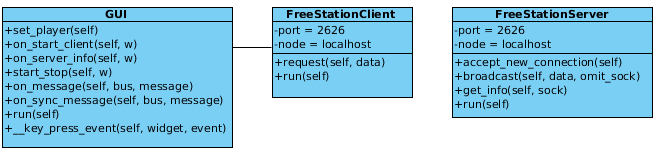
\includegraphics[width=460px]{src/img/class-diagram.png}
        \caption[Diagrama de clases]
          {Diagrama de clases}
    \end{center}
\end{figure}

El primer prototipo es funcional y pretende demostrar la intención de
comunicación de datos entre cliente y servidor.

\subsection{Fase 2 - Migración a ICE}

Debido a la complejidad incremental de usar sockets para un desarrollo más
avanzado, se desecho la idea en una tutoría de proyecto en favor de utilizar una
tecnología de distribución de objetos distribuidos. Tras varias comparativas, se
decidió usar \acs{ICE} por su versatilidad y comodidades en el desarrollo con
Python y otras ventajas explicadas anteriormente (véase
apartado ~\ref{sec:ZeroICE}).

Se dedica tiempo de estudio a ICE leyendo la documentación oficial\cite{Spr12} y
formas de implementación en Python.
Se realizan pequeñas pruebas y prototipos de ejemplos con el manual de David
Vallejo sobre ICE\cite{Val06}. Se acuerda establecer un listado de componentes
necesarios para la aplicación.

\subsection{Fase 3 - Implementación widgets}

Se implementa una lista de componentes (widgets) tentativa para el cliente de
\emph{FreeStation}. Esta lista es inicialmente un prototipo de widgets que
podrían resultar útiles en siguientes iteraciones de proyecto. Se planifica en
posteriores iteraciones estudiar la viabilidad de implementar los widgets más
detalladamente o con características más avanzadas.

Algunos de los widgets:

\begin{itemize}
    \item *1 - \textbf{MountDetector}: Detecta la presencia de unidades USB
    (montaje/desmontaje) y recopila la información del nombre de la unidad, espacio disponible y total.
    \item*2 - \textbf{MountInfo}: Configura una interfaz a partir de los datos
    de MountDetector con una barra de progreso para mostrar el espacio disponible/total.
    \item*3 - \textbf{VideoArea}: Carga un vídeo en reproducción continua y se
    activa en pantalla completa cuando FreeStation pasa a modo idle.
    \newpage
    \item4 - \textbf{SliderArea}: Paneles informativos deslizantes con
    información para banners, transparencias, etc.
    \item*5 - \textbf{Browser}: habilita la navegación de una pagina web externa
    o documento html local.
    \item*6 - \textbf{BrowserView}: renderiza templates según la vista (MVC:
    Modelo Vista Controlador) y trata con la lógica de la información proporcionada por el componente Browser.
    \item*7 - \textbf{GUI}: Inicializa la aplicación y lee los componentes
    habilitados para su carga, lanzándolos posteriormente.
    \item8 - \textbf{CategoryArea}: Zona de información de listas verticales de
    categorías de información.
    \item*9 - \textbf{MenuActionsArea}: menú formado por flechas de
    anterior/siguiente/inicio para interactuar con las posibles zonas
    \item10 - \textbf{ItemArea}: Muestra la información sobre algún elemento
    (puede ser software, documento, etc) con elementos como logo, descripción, dependencia, título.
    \item*11 - \textbf{LogoArea}: Carga un logo por defecto para la institución,
    universidad, escuela, oficina de turismo, ayuntamiento, etc.
    \item*12 - \textbf{TitleDisplay}: Carga un título central por defecto para
    la institución, universidad, escuela, oficina de turismo, ayuntamiento, etc
    \item13 -\textbf{ClockArea}: Renderiza la hora actual.
\end{itemize}

Nota: Los componentes marcados con * delante son funcionales e implementados en
dicha fase.

La implementación en esta fase conlleva alrededor de tres semanas al tener un gran
componente de desarrollo e investigación por cada widget planteado.

\newpage

\subsection{Fase 4 - Clases abstractas}

Puesto que la implementación esta hecha en Python, se intentan utilizar clases
abstractas como sugerencia, aunque no tiene mucha aplicación ya que cada
componente tiene su lógica por separado y estos heredan (especializaciones) de
las clases necesarias, o tienen asociaciones y dependencias con otros
componentes (por ejemplo
\emph{MountDetector}<->\emph{MountInfo}<->\emph{Gui}<->\emph{FreeStationApp}).

Aparte se investiga que las clases abstractas en python, son
pseudo-implementadas con \emph{RaiseError} o \emph{Exception}, pero no tienen
una sintaxis definida propia (como Java o PHP), sino como metaclases. Se desecha
la idea de implementar un patrón de herencia basado en clases abtractas, 
aunque no se descarta la posibilidad de usar alguna cuando sea más necesario.

\subsection{Fase 5 - Migración de GTK2 a GTK3}

El desarrollo del código para interfaces empezó en las primeras iteraciones
basado en la biblioteca GTK2. En el proceso, la mayoría del software relacionado
con la plataforma GTK empezó a basarse en la nueva biblioteca GTK3 (véase
~\ref{sec:GTK}).

A corto y medio plazo la estimación era que podrían producirse problemas de
compatibilidades y abandono de la plataforma GTK2 o pequeños fallos que no
fueran corregidos. La ventaja de utilizar la nueva biblioteca en GTK3 era una
mayor potencia y versatilidad de desarrollo, pero podrían producirse fallos no detectados.

Se opta por migrar todo el código anterior de widgets de GTK2 a GTK3, ya que
para el binding de Python existe un gran aumento de rendimiento y por lo general
es más fácil de escribir el código en la nueva versión.

Este proceso dura aproximadamente una semana y media y requiere de consultas en
listas de correo de desarrollo de GTK y preguntas a desarrolladores en IRC para
las opciones más avanzadas en la migración. En la migración se utilizado el
tutorial de migración de GTK (véase sección \cite{Gno12}).

\newpage 

\subsection{Fase 6 - Detección USB}

En esta iteración se trata de completar, optimizar y añadir mas funcionalidad a
los widgets encargados de la detección de USB. Se estudia el posible uso de DBus
(véase ~\ref{sec:DBus}) como principal elección para comunicación de eventos por
mensajes de nuevos dispositivos hardware USB.

Para la implementación se desarrollan dos widgets. El primero llamado
\emph{MountDetector} detecta nuevos dispositivos de almacenamiento USB y
recopila los datos en crudo. Una vez dispone de los datos, los envía a un segundo widget
llamado \emph{MountInfo} donde se procesan los datos para impresión y
tratamiento de la interfaz. Este widget sera el encargado de tratar con la interfaz principal de
la aplicación cliente.

La implementación resulta tediosa al no disponer de una documentación lo
suficientemente clara y ejemplos basados en python. A través de ejemplos en C
y visualización de implementaciones de otros programas se realiza la
implementación. La migración del código GTK2 a GTK3, resulta satisfactoria,
aunque algunas primitivas nativas de la biblioteca cambian radicalmente.

\subsection{Fase 7 - Problemas con Gstreamer}

Para la realización e implementación de un widget de vídeo se empezó el 
desarrollo del widget \emph{VideoArea}. Este widget sería capaz de mostrar un
vídeo, reproducirlo en bucle o pasar a modo idle en pantalla completa cuando no existiera interacción con la aplicación
principal.

Se decidió usar la biblioteca \emph{Gstreamer} (véase
~\ref{sec:Gstreamer}) en su versión 0.10. Se implemento la reproducción sin
bucle y sin modo idle en GTK2. Posteriormente en la migración del código a GTK3,
se detectó que los mensajes emitidos en la finalización del flujo de vídeo no 
eran emitidos, lo que imposibilitaba implementar la característica de integrar
el widget de la ventana de vídeo con otros widgets en la misma ventana.

Esto resultaba en la aparición de dos ventanas por separado y como consecuencia
el modo completo de pantalla pasaba a modo normal. 

\newpage

Se intento llegar a una
solución intermedia donde mezclar el widget de GTK2 funcional con el resto de 
widgets portados a GTK3, pero seguían produciéndose
conflictos con la biblioteca interna GObject.

Se reporto un bug en proyecto Gnome
(véase Bug \#631901\footnote{Bug \#631901 Gnome:
\url{https://bugzilla.gnome.org/show_bug.cgi?id=631901}\label{ftn:GnomeBug}})
con el fin de que los desarrolladores tuvieran consciencia del problema y se 
presentara una arreglo o solución próxima. La iteración se finaliza a la 
espera del arreglo para una próxima versión 0.11 de Gstreamer (considerada 
1.0) que pueda solucionarlo. El problema principal esta en la migración interna
de gst-python (binding de python para Gstreamer) al nuevo \acf{GI} de GTK3.

\subsection{Fase 8 - POC de ICE}

Tras la investigación y formación en la documentación de ICE se decide realizar
un desarrollo commo prueba de concepto (\acs{POC}\label{acro:POC}) para probar
las llamadas y la ejecución de ICE.

Se desarrolla una clase cliente llamada \emph{FreeStationClient} y otra backend
llamada \emph{FreeStationServer} como fue explicado en la sección de
arquitectura ~\ref{sec:backendice}. Se realiza un vídeo ilustrativo como ejemplo
de funcionamiento de las conexiones y pruebas de rendimiento.

En el vídeo se trata la aplicación en ejecución en modo pantalla completa para
el cliente con algunos widgets se hace la prueba de interacción insertando un
USB de 1 GB para su detección. Se acuerda una nueva reunión para visualizar la
demo en directo, aumentar/modificar la lista de widgets, enfocar las siguientes tareas a realizar
y comentar cualquier otra duda.

Se propone realizar pequeños artículos en el blog personal para ir comentando el
progreso y tener una memoria de las iteraciones.

\newpage

\subsection{Fase 9 - Reemplazar Webkit por Gecko}

Para la visualización de páginas webs embebidas como widget en la aplicación cliente
se debería elegir un motor de renderizado de páginas webs.

Las alternativas disponibles bajo un binding de python eran:

\begin{itemize}
  \item \textbf{Gecko}: el motor de renderizado usado por Firefox. Usa la
  biblioteca gtkmozembed y estaba basado para funcionamiento con GTK.
  \item \textbf{WebKit}: el motor de renderizado de Google Chrome, Safari, etc.
  Estaba adaptado a GTK mediante la biblioteca WebKitGTK+.
\end{itemize}

Respecto a gtkmozembed el proyecto no tenía un ritmo de actualización activo, ya
que no disponía de actualizaciones desde 2005. Desde las versiones de GTK 2.2X
no tenía buen soporte y no era perfectamente funcional. Para GTK3 no existía
ninguna actualización que permitiera ejecutar su código sin fallos.

Debido a ello, se descarto usar gtkmozembed por su bajo soporte. Por lo tanto,
WebKit basado para Gnome con el nombre de biblioteca
\emph{WebKitGTK}\footnote{WebKitGTK: \url{https://live.gnome.org/WebKitGtk}}
tenia un soporte bastante decente con actualizaciones frecuentes. El soporte
ofrecido por Ubuntu parece consolidarse al utilizar la biblioteca en varias 
aplicaciones de la distribución.

Se propone la investigación del funcionamiento de algunas aplicaciones como el
Centro de Software de Ubuntu para ver el funcionamiento de la biblioteca y
principales usos.

\subsection{Fase 10 - Watchdog y Webkit}

En la mejora del \emph{Watchdog} se implementa finalmente siendo totalmente
funcional (véase sección ~\ref{sec:watchdog}). Se observa un problema en el
reinicio de la aplicación que parece interferir en el widget de Webkit.

\newpage

El problema reside en la biblioteca ya que realiza un lock (bloqueo) interno
para renderizar en el hilo principal. Esto provoca un mal renderizado del widget
de Webkit exclusivamente al utilizar el \acs{GDK}\label{acro:GDK} lock

Se observan referencias al problema en listas de correo\footnote{The GDK Lock:
\url{http://pvanhoof.be/blog/index.php/2007/08/04/the-gdk-lock}\label{ftn:GDKlock}}
y fuentes oficiales de webkit\footnote{What supposed to hold the GDK in calls from WebKit/gtk/WebCoreSupport:
\url{https://lists.webkit.org/pipermail/webkit-gtk/2011-August/000651.html}\label{ftn:WebkitLOCK}}.
Como conclusión se deduce que Webkit no libera correctamente el lock 
establecido y provoca que el objeto del widget del Browser se quede congelado.

Al ser previsto para solucionar en próximas versiones se decide seguir con la
implementación actual ya que es la única alternativa para renderizar páginas
webs como widget con threads. Este enfoque es necesario por el watchdog que
lanza las aplicaciones como hilos.

El watchdog en las primeras iteraciones se implemento con el módulo 
\emph{multiprocessing} y la clase \emph{Process}. De esta forma se realizaban
nuevos procesos hijos a partir de forks del watchdog. Era funcional esta
implementación, pero al reiniciar la aplicación, existían problemas con 
punteros de GTK que no eran liberados desde el
binding de Python. Esto provocaba errores como que las X eran un
recurso temporalmente en uso.

Se intento investigar el problema bajando el código de \emph{XLib} y se detecto
que la función que procesaba el binding era la función \emph{XOpenDisplay} y
devolvía un XIO error. Debido a la complicación del binding en GTK escrito en
C++ y tener que realizar compilaciones con demasiadas dependencias del 
entorno GNOME se desecho al salirse de los objetivos de la iteración y 
extensión del proyecto.

De esta forma se optó por el módulo de threadings e implementarlo como hilos
con un funcionamiento correcto, excepto por el objeto de Webkit comentado
anteriormente. También se intento previamente bajar el repositorio actual de
código de Webkit (3.5 GB) y se encontró la parte de desarrollo de GTK para 
WebKit\footnote{Webkit source para GTK:\\
\url{http://svn.webkit.org/repository/webkit/releases/\\WebKitGTK/webkit-1.6.1/Source/WebKit2/}\label{ftn:WebkitSourceGTK}} 

\newpage

La extensión era bastante grande para detectar el XIO error y se abandonó aún a
pesar de consultar algunos manuales para modificaciones de GTK\footnote{HackingGtk:
\url{http://trac.webkit.org/wiki/HackingGtk}\label{ftn:HackingGtk}}.

\subsection{Fase 11 - Punto de entrada con GTKApplication}

\emph{GtkApplication}\footnote{GtkApplication:\\
\url{http://developer.gnome.org/glibmm/unstable/\\classGio\_1\_1Application.html}\label{ftn:GtkApplication}}
es una clase para administrar todos los aspectos importantes de
una aplicación GTK. Esta ideada para reforzar el concepto de encajar en la
idea de aplicación modelo.

\emph{GtkApplication} realiza la inicialización GTK+ por defecto, asegura la
unicidad de ejecución de la aplicación, administración de sesiones y provee integración con
scripts y escritorio. Permite exportar acciones y menú a ventanas de alto nivel
en el ciclo de desarrollo de la aplicación. La versión inicial desarrollada
usaba \emph{GtkApplication} para aprovechar las ventajas expuestas.

Debido a su novedad e implementación reciente en GTK 3 surgieron problemas en el
desarrollo. En concreto, la aplicación mediante \emph{GTKApplication} creaba un
objeto que recibía señales. Una de las señales permite interactuar con la aplicación
una vez que finaliza. En este caso la señal invocada por el método $release()$
debería terminar la aplicación, pero dejaba el thread como zombie. Esto es
debido a que la clase \emph{GTKApplication} actúa como un
constructor/destructor, pero no liberaba correctamente la última instancia.

Tras investigar el problema, parece un problema conocido por los desarrolladores
de GTK\footnote{Bug 637445 - Finish Gtk::Application:\\
\url{https://bugzilla.gnome.org/show\_bug.cgi?id=637445\#c17}\label{ftn:GtkBugzilla}}.
En el momento de la iteración, desde GTK no estaban seguros de la especificación final de la implementación y con previsiones de avanzarla o terminarla en Gnome
3.2\footnote{Gtk::Application punted to gtkmm 3.2:\\
\url{http://old.nabble.com/Gtk::Application-punted-\\to-gtkmm-3.2-td31220771.html}\label{ftn:Application-punted}}.
Debido a estos problemas, se aplaza y desecha la implementación actual con \emph{GtkApplication} y se implementa como un thread lanzado por la clase
watchdog.

\newpage

\subsection{Fase 12 - Widgets posicionados relative/absolute}

Se investiga la forma de crear widgets mediante posicionamientos relativos y
absolutos. Se mira el funcionamiento de Ogre3D\footnote{Ogre3D:
\url{http://www.ogre3d.org}} y su implementación como referencia. Se observa las
características ofrecidas en Glade\footnote{Glade \url{http://glade.gnome.org}} 
y por GTK para realizar los posicionamientos mediante ficheros XML.

\subsection{Fase 13 - Carga por XML}

En esta iteración se concreta y modela la especificación de carga para los
widgets. Se define una especificación basada en XML. Este enfoque permite
utilizar las definiciones para manejar eficientemente tipos de datos 
complejos, etiquetados o ocurrencias de widgets.

Se establece una primera definición con las propiedades y elementos que pueden
disponer como base los widgets. Para la carga de widgets mediante XML se
implementa una clase llamada \emph{WidgetLoader} vista en la sección de arquitectura
~\ref{sec:widgetloader}.

Esta delega la tareas de carga un parseador XML (XMLParser) y detecta los
widgets con sus respectivas configuraciones. Una vez que los datos son
procesados, se cargan en la estructura del WidgetLoader permitiendo controlar 
los fallos de análisis o duplicidades.

\subsection{Fase 14 - Arranque del backend}

Se prueba un posible arranque del backend por medio del un servicio en el
arranque por init.d. Se desecha la idea ya que requiere intervención mediante
consola de comandos y se piensa una mejor solución.

Se implementa un servicio para arrancar en el servidor los
servicios de ICE y que respondan a un frontend en PHP. Esto evita la interacción
por consola y una gran comodidad y facilidad de gestión desde el frontend web.

\newpage

La interfaz web permite conectar al cliente y crear el servidor en ejecución. La
interfaz web del servidor se planifica para mejor desarrollo, con el fin de 
que el caso de explotación pueda hacer un ejemplo simple de los
widgets y utilice distintos datos cargados como posicionamientos
relativos o absolutos, ancho y alto y configuraciones personalizadas.

\subsection{Fase 15 - PyUnit testing}

Para las pruebas del proyecto se empezó realizando un pequeño conjunto de
pruebas de test unitarios. Dado que la mayor parte del proyecto estaba escrito
en Python se eligió el framework PyUnit. En su inicio se cubrieron los test para
secciones más críticas y consolidadas como \emph{Watchdog}, 
\emph{FreeStationApp} y \emph{BrowserView}. El posterior objetivo no era hacer
un completo code coverage, pero si bastante avanzado.

En posteriores iteraciones se valoró cubrir las clases \emph{WidgetLoader} y
\emph{XMLParser} por su repercusión de errores en la detección de archivos XML y
asegurar un buen funcionamiento de la aplicación en la parte cliente.

Debido a la falta de tiempo se pospone la escritura de artículos técnicos en el
blog personal prioritizando el desarrollo y documentación del proyecto. Asimismo
los problemas surgidos con GTK y derivados se retrasan algunas partes del 
desarrollo investigando soluciones.

\subsection{Fase 16 - Mejora del POC de ICE}

Se mejora el diseño de la aplicación cliente y servidor con la conexión ICE. Se
hacen llamadas mediante especificaciones de ficheros .ice (slice), mejora del 
tratamiento de excepciones y reescritura del código para mejorar la
encapsulación.

La configuración del cliente y servidor se hace en tiempo de ejecución y se
dedica la gran parte del tiempo de iteración a comprender mejor el
funcionamiento interno de las funciones de ICE.

\newpage

\subsection{Fase 17 - Mejora widget VideoArea en GTK3}

En anteriores iteraciones el widget de \emph{VideoArea} fue desarrollado pero se
necesitaban nuevas funcionalidades como reproducción en bucle y empotrado del
widget en ventanas GTK.

En esta iteración se consiguió hacer funcionar la reproducción en bucle en GTK3
debido a que parte del bug que fue reportado funcionaba mejor con la versión
0.11 de GStreamer. También se modificó la disposición del widget y permitía el
empotrado en una ventana independiente que podía asociarse con otros widgets. La
reproducción de ficheros locales e incluso url externas era funcional. Se
realizan pruebas con el trailer de Sintel\footnote{Sintel:
\url{http://www.sintel.org}}\footnote{Sintel trailer 480p:
\url{http://docs.gstreamer.com/media/sintel\_trailer-480p.webm}} en formato WebM\footnote{WebM Project:
\url{http://www.webmproject.org}}. 

Como información para la reproducción mejorada en Gstreamer se usan
documentación y tutoriales procedentes de la Guía de Novacut\footnote{Novacut:
\url{http://novacut.com}} para migraciones Gstreamer 1.0\footnote{Guía Novacut
para GStreamer:\\https://wiki.ubuntu.com/Novacut/GStreamer1.0}

Por otro lado, se confirma la liberación de GStreamer 1.0 para principios de
Octubre como fecha tentativa. Esta nueva versión sera empaquetada por defecto en
todas las versiones de Ubuntu 12.10 y posteriores lo que asegura un buen
funcionamiento de la aplicación siguiendo la especificación actual.

\subsection{Fase 18 - Intento de solución para WebKit}

En esta iteración se propone solucionar el problema con los threads de WebKit.
Tras varios días de intentos infructuosos se obtienen un resultado como
conclusión. Webkit no permite el uso con threads fuera del hilo principal.

El motivo es que su implementación no es "thread safe" y solo puede
usarse desde el hilo principal de la aplicación. El problema afecta en el
desarrollo del watchdog desde que es lanzado como aplicación principal en un
thread para \emph{FreeStationApp} y esta a su vez lanza los hilos
correspondientes en la aplicación, uno de ellos el correspondiente a WebKit.

Puesto que no esta dentro de uso del thread principal, la primera vez que es
iniciado WebKit funciona sin problemas, pero posteriores reinicios con el
Watchdog no habilitarán el renderizado de Webkit. Para ello es necesario
reiniciar por completo el watchdog. El problema de Webkit viene de la
cancelación del render en uno de sus cuatro estados posibles al renderizar una
aplicación web: \emph{provisional->commited->finished->rendered}. En el momento
del render, el GDK lock hace imposible utilizarlo y se hacer un rollback del
estado del render pintando un widget en negro vacío. 

La confirmación de esta situación viene del mensaje:\\
\url{http://markmail.org/message/
4dwft6s6g6ptavj6}

En concreto, se establece el problema con las líneas:

\begin{quote}
    \small Webkit is not thread-safe. External processing  
            on a secondary thread is OK, but any calls into the DOM will have  
            to happen on the main thread.
\end{quote}

De esta forma los contenidos se llegan a cargar, pero no se renderiza el DOM ya
que debe realizarse en el thread
principal\footnote{GDK\_Threads: \\
\url{http://www.yolinux.com/TUTORIALS/GDK\_Threads.html}}

\subsection{Fase 19 - Refactorizado de widget para propiedades}

Para la carga del \emph{WidgetLoader} se debían detectar propiedades que el
widget incorporará en el formato de la etiqueta $<properties>$ del fichero XML.

Se refactoriza el código del mismo para que se admitan propiedades del alto,
borde y algunas propiedades más en algunos widgets básicos como el
\emph{LogoArea}, \emph{TitleArea} y \emph{FeedArea}.

\newpage

\subsection{Fase 20 - Implementación de widget lector RSS}

Como consecuencia de la anterior iteración se hace necesaria la implementación
de un widget que realice lecturas de suscripciones RSS. En el widget se utiliza
la biblioteca feedparser de python y se añade una imagen de feed como icono.

Se configura con lector de título RSS, personalización de cada entrada y una
ventana con scroll. El lector tiene en cuenta las entidades HTML para limpiar
caracteres no adecuados en su representación.

\subsection{Fase 21 - Theming de GTK}

Tras la realización de un conjunto bastante amplio de widgets para
\emph{FreeStation} se decide investigar el theming con GTK para mejorar la
apariencia de la aplicación y crear un caso de explotación con una paleta de
colores y diseño similar a la UCLM.

Los principales problemas que surgen con el theming es que no existe mucha
información al respecto ni ejemplos avanzados. Se decide investigar en el código
fuente de GTK para realizar algunas propiedades que no estaban completamente
claras y por otro lado en el binding de GTK generado para python.

El theming es posible realizar a partir de ficheros de estilos CSS básicos. Pero
la mayoría de los modelos renderizados con GTK son cuadrados y no se puede
aplicar bordes redondeados de forma sencilla. Se prueba con la propiedad
border-radius pero no es efectiva. Buscando ejemplos similares en código fuente
del centro de software Ubuntu se realizarán algunos cambios significativos, pero
no resulta en la apariencia esperada.

La apariencia final tiene como resultados los expuestos en la sección de
arquitectura ~\ref{sec:casestudygtk}.

\newpage

\subsection{Fase 22 - Investigación de tecnologías basadas en CouchDB}

Puesto que en la anterior iteración el resultado no era el esperado se
investigan nuevas tecnologías punteras que permitan una mejor apariencia de la
aplicación y efectos de animación. En una sesión presencial se comenta la
posibilidad de usar CouchDB con una interfaz web en Webkit que comunique con GTK. Se dedica una semana y media para
comprender la tecnología y realizar pequeños ejemplos funcionales.

\subsection{Fase 23 - Migración del proyecto completo a CouchDB}

Los resultados en los ejemplos funcionales son muy prometedores y aunque resta
poco tiempo de desarrollo para finalización del proyecto se decide
reimplementarlo completamente (aprovechando los módulos posibles) para que estos
sean renderizados con CouchDB. Esto conlleva varias semanas de trabajo y
reescribir parte de la documentación y test existentes.

\subsection{Fase 24 - Mejoras en la implementación}

Se finaliza la implementación de la parte de copia de USB en CouchDB y cambios
en la presentación de los contenidos (flechas de botones en jerarquía) y
mejorado el aspecto visual de la parte de noticias.

Se termina la implementación de la parte de copia a usb y realizan algunos
cambios de presentación (añadida una flecha en los botones de jerarquía) y 
mejorada la sección de noticias. Se consigue acoplar perfectamente todas las
bibliotecas antiguas en freestation y ya no es necesario ejecutarlo como
proyecto aparte del basado en GTK. Se integra la funcionalidad completa en un
nuevo widget llamado \emph{UclmDemoCouch}

\subsection{Fase 25 - Reescritura a Python 3}

El cambio a CouchDB también implica la reescritura del código de python 2.7 a
python 2.7, salvo el cliente en Ice que no dispone de soporte para Python 3 y se
ejecuta de forma independiente en Python 2.7

\newpage

\subsection{Fase 26 - Creación de USB Bootable}

La característica a implementar del USB Bootable da algunos problemas al no
conocer una documentación existente por línea de comandos y durante la migración
de CouchDB queda relegada hasta poder investigar más la tecnología. Se valora la
posibilidad de no incluirlo en la implementación por falta de tiempo.

Se mejoran los mensajes de error en la copia de USB si no existe espacio en
disco suficiente y se propone como implementación futura que previamente se
realice un cálculo de los ficheros para valorar el tamaño final a copiar. Se
habilita un flag o bandera en el código para habilitar el caso de explotación 
en GTK3 o CouchDB.

\subsection{Fase 27 - Contribuciones a bibliotecas de CouchDB}

Tras la implementación completa del proyecto en \emph{CouchDB} y el uso de una
biblioteca de ejemplo llamada
\emph{userwebkit}\footnote{userwebkit: \url{https://launchpad.net/userwebkit}}
se decide incorporar la biblioteca integrada y adaptarla a las necesidades
específicas de \emph{FreeStation}.
Esta biblioteca es una variedad de framework en \emph{Webkit} para la aplicación
Novacut\footnote{Novacut: \url{https://launchpad.net/novacut}}.

Puesto que la biblioteca esta orientada a la aplicación \emph{Novacut} incorpora
por defecto un recolector de imágenes del sistema llamado
\emph{dmedia}\footnote{Dmedia: \url{https://launchpad.net/dmedia}}. Por este
motivo se refactoriza la biblioteca userwebkit para desacoplar las
funcionalidades e integrar sólo las partes necesarias en FreeStation. En
concreto se incluyen las mejoras en el widget \emph{BrowserView} que se
desarrollo para el uso de \emph{WebKit}.

En el proceso de refactorización se consigue crear una funcionalidad que permite
interceptar la consola de mensajes de WebKit. Aunque no era objetivo de
FreeStation si complementaba su funcionalidad. Capturando los mensajes de la
consola se podían tratar bien los errores y mensajes lanzados por WebKit.

Como resultado se realizó un parche de la funcionalidad para que el autor de
las bibliotecas novacut, dmedia y userwebkit pudiera incorporarlo en su proyecto.

El bug \#1023770\footnote{Bug \#1023770 Launchpad
\url{https://bugs.launchpad.net/userwebkit/+bug/1023770}} fue reportado y adjuntado el
parche\footnote{Merge proposal(parche): \\
\url{https://code.launchpad.net/~shakaran/userwebkit/webkit-console/+merge/118470}}.
Su autor agradecio enormemente la contribución en una mención en
Google+\footnote{Mención Google+:
\url{https://plus.google.com/u/0/114471118004229223857/posts/7287aAdYNup}}

\subsection{Fase 28 - Prueba de funcionalidades en CouchDB}

Como prueba de la funcionalidad se comprobó que los eventos de CouchDB se
emitían y capturaban bien, aunque en el proceso de detecto que no permitía
reevaluar contenido javascript en las peticiones, por lo que todo el código
javascript debería ser previamente incluido y activar funciones con eventos.

Las peticiones Ajax no eran \emph{crossdomain} por lo que no se permitía obtener
datos de otros servidores que no fueran localhost. Tampoco se podían cargan
imágenes en local, sólo permitía imágenes externas. Se solucionó este problema
añadiendo una directiva en webkit para carga de archivos locales.

Se procede a rellenar el contenido de las restantes secciones del ejemplo del
caso de explotación y se realiza un vídeo para la evaluación del tutor.

\subsection{Fase 29 - Desarrollo USB Bootable con UnetBootIn}

Tras analizar la funcionalidad de \emph{unetbootin} se valora la posibilidad de
hacer un wrapper o adaptador del código C++ a python.

Posteriormente en la documentación del proyecto (wiki)\footnote{unetbootin:
\url{http://sourceforge.net/apps/trac/unetbootin/wiki/commands}} se
descubren funcionalidades por línea de comandos que permiten generar USB
bootables a partir de ficheros .iso.

\newpage

Un ejemplo de comando sería:

\begin{lstlisting}[language={Bash}, texcl=false, label={lst:unetbootin},
caption={Copia de fichero .iso con unetbootin}] 
unetbootin method=diskimage isofile="/path/file.iso"
\end{lstlisting}

Debido a la falta de tiempo, se pospone y se decide dedicar el resto de tiempo
disponible a terminar y mejorar la documentación del proyecto.

\section{\uppercase{Recursos y costes}}

En este apartado e enumeran y describen el conjunto de diferentes recursos
principales y la especificación de los mismos, tanto temporales como económicos,
en conjunto a herramientas de apoyo y análisis para el proyecto de fin de carrera.

Se evalúan sus características principales y se detalla la planificación y
presupuesto inicial y final (estimados) del mismo.

\subsection{Presupuesto y planificación iniciales}

\subsubsection{Presupuesto inicial}

Se parte de una planificación inicial desde Septiembre de 2011, elaborada al
comienzo del proyecto basada en modelos, conceptos teóricos y la experiencia en el 
desarrollo de proyectos similares. Se estima inicialmente el proyecto para una
duración de 4 meses para entrega en Febrero de 2012.

Durante el desarrollo la incorporación de nuevas características y ampliación de
requisitos llevan a prolongar la duración del proyecto durante 4 meses más
hasta Junio de 2012. Como resultado de problemas en el desarrollo e
incorporación de nuevas características se amplía como fecha definitiva y no
prorrogable hasta Septiembre de 2012. 

Por tanto la duración del mismo conlleva
un año de trabajo.

\newpage

\subsubsection{Coste de personal}

En este apartado, se detalla el proceso operacional seguido para la 
obtención del salario por hora de trabajo de los diferentes roles 
participantes en el proyecto. Los resultados obtenidos se presentan,
posteriormente, en forma de tabla.

\begin{table}[ht]
    \centering
    \begin{tabular}{|l|l|}
      \hline
      \multicolumn{2}{|c|}{Estimación horas laborables} \\
      \hline
        Días laborables / mes &  20 \\
        Horas trabajadas / día & 6 horas \\
        Horas trabajadas / mes & 120 horas \\
      \hline
    \end{tabular}
    \caption{Estimación horas laborables por día y mes}
     \label{tab:hourestimation}
\end{table}

En el presupuesto inicial se estimo un salario neto por persona al mes (el
mismo para todos los roles) de 1200 € como ingeniero junior.

Aplicando los costes de recursos humanos:

\begin{table}[ht]
    \centering
    \begin{tabular}{|l|l|}
      \hline
        \multicolumn{2}{|c|}{Costes por recurso humano} \\
      \hline
       IRPF (20\% sobre el salario neto) & 240,00 \\
       Seguridad Social (40\% sobre salario neto + IRPF) & 576,00 \\
       Salario bruto por persona / mes: Salario neto + IRPF + Seguridad Social &
       2016 \\
       Meses laborables & 11 meses \\
       Horas en un año & 1760 horas \\
      \hline
    \end{tabular}
    \caption{Estimación horas laborables por día y mes}
     \label{tab:hourestimation}
\end{table}

Esta tabla refleja por tanto un coste bruto por persona y hora igual al salario
bruto por persona y año / horas en un año. Total 16,03 €/hora.

Suponiendo un salario bruto por persona y año (suponemos 14 pagas): 28224 €

\subsubsection{Equipos informáticos}

Como fue explicado en la sección \label{sec:harware} fue necesario un coste
Hardware en equipos y servidores. 

\newpage

Las siguientes tablas detallas una estimación del coste de los mismos:

\begin{table}[ht]
    \centering
    \begin{tabular}{|l|l|}
      \hline
      \multicolumn{2}{|c|}{Costes por equipos} \\
      \hline
       Acer Aspire Ethos 5943G (laptop) & 1299,00 € \\
       Acer Aspire One (netbook) & 299,00 €\\
       Compaq Presario C700 & 469,00 €\\
       HP 620 & 699,00 €\\
       Sobremesa & 999,00 €\\
       \hline
    \end{tabular}
    \caption{Costes por equipos}
     \label{tab:hwstimation}
\end{table}

El total de la tabla ~\ref{tab:hwstimation} asciende a 3765 €.

\begin{table}[ht]
    \centering
    \begin{tabular}{|l|l|}
      \hline
      \multicolumn{2}{|c|}{Costes servidores} \\
      \hline
       Servidor dedicado (OpenVZ, 512 MB RAM) & 27 € / mes\\
       Servidor dedicado (VMWare, 8 GB RAM) & 150 € / mes\\
      \hline
    \end{tabular}
    \caption{Costes por servidores}
     \label{tab:serverestimation}
\end{table}

El total de la tabla ~\ref{tab:serverestimation} para un año asciende a 2124 €.

\subsubsection{Licencias}

\begin{table}[ht]
    \centering
    \begin{tabular}{|l|l|}
      \hline
      \multicolumn{2}{|c|}{Costes por licencias} \\
      \hline
       GTK  & 0,00 € / año \\
       VMWare & 225,63€ / año\\
       OpenVZ & 0 € / año\\
       Ubuntu 12.10 & 0 € /año\\
       CentOS 6.8 & 0 € /año\\
       GStreamer & 0 € /año\\
       Zero C ICe & 0 € /año\\
       Gimp & 0 € /año\\
       Otros & 0 € /año\\
      \hline
    \end{tabular}
    \caption{Costes por licencias}
     \label{tab:licensestimation}
\end{table}

El total de la tabla ~\ref{tab:licensestimation} asciende a 225,63 €.

\newpage

\subsubsection{Material fungible}

\begin{table}[ht]
    \centering
    \begin{tabular}{|l|l|}
    \hline
        Descripción & Coste (Euros) \\
        Material de impresión & 150,00\\
        Material de oficina & 55,00 \\
      \hline
    \end{tabular}
    \caption{Coste material fungible}
     \label{tab:matfungible}
\end{table}

El total de la tabla ~\ref{tab:matfungible} asciende a 205,00 €.

\subsubsection{Resumen de costes del proyecto}

El coste final del presupuesto inicial del proyecto, partiendo de los datos
obtenidos en los apartados anteriores serían.

\begin{table}[ht]
    \centering
    \begin{tabular}{|l|l|}
    \hline
        Descripción & Coste (Euros) \\
        Recursos humanos & 28224,00 €\\
        Coste hardware & 3765\\
        Coste servidores & 2124 €\\
        Licencias &  225,63 € \\
        Material fungible & 205,00 € \\
      \hline
    \end{tabular}
    \caption{Resumen costes del proyecto}
     \label{tab:totalpresupuesto}
\end{table}

El Total de presupuesto inicial mostrado por la tabla
~\ref{tab:totalpresupuesto} asciende a 34453,63 €.

\subsection{Planificación final del proyecto}

Para contabilizar y representar las iteraciones y el tiempo de desarrollo. Se
creo un diagrama Gantt correspondiente a la
planificación inicial y final que se realizó para el desarrollo del sistema \emph{FreeStation}.

\newpage

\begin{figure}[ht]
    \begin{center}
        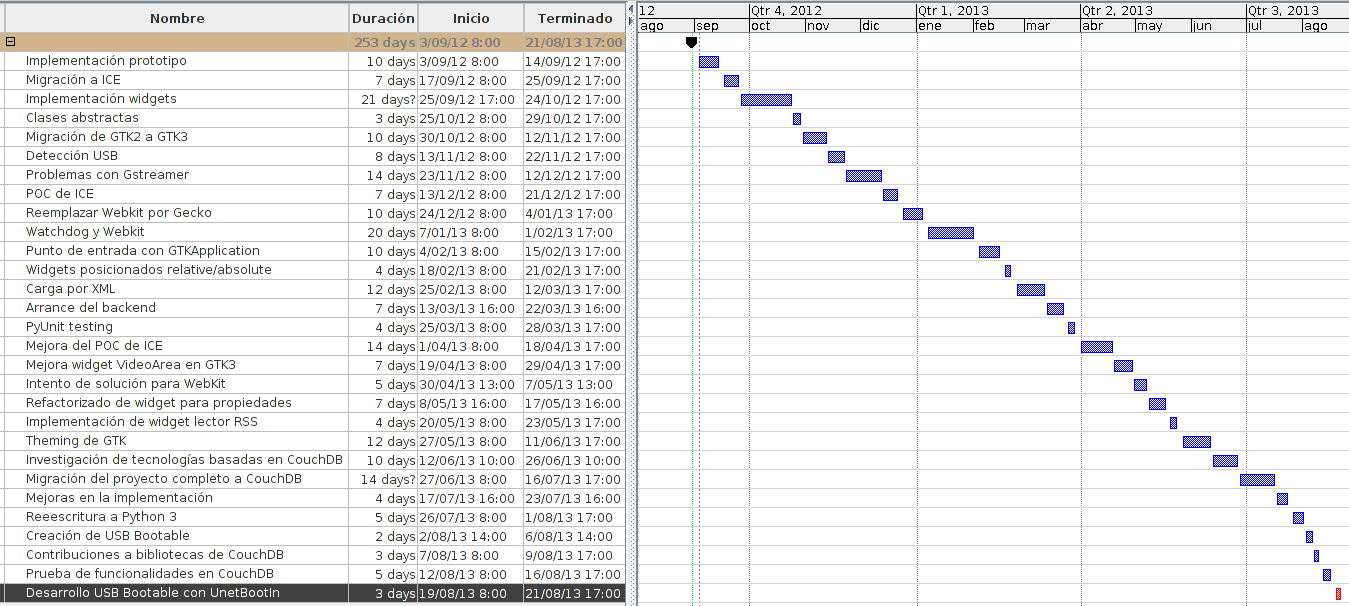
\includegraphics[width=425px]{src/img/diagrams/gant-diagram.png}
        \caption[Diagrama de Gantt]
          {Diagrama de Gantt}
          \label{fig:gantdiagram}
    \end{center}
\end{figure}

La figura ~\ref{fig:gantdiagram} muestra la planificación desde principios de
Septiembre de 2011 a finales de Agosto de 2012. 

\emph{Nota}: se ha utilizado la herramienta OpenProj\footnote{OpenProj:
\url{http:\\openproj.org}} para realizar la estimación de costes y diagrama de
Gantt.

La estimación total se ha hecho siguiendo horarios laborales de 8:00 a 17:00 de
Lunes a Viernes con una duración total de 253 días laborables en aproximadamente
unas 50 semanas de trabajo.

\subsubsection{Coste final del proyecto}

Siguiendo la figura ~\ref{fig:gantdiagram} y haciendo un
recuento del tiempo empleado en el desarrollo del proyecto se han necesitado 
253 días laborables, a un precio estimado de 40 € la hora de
ingeniero durante 6 horas al día, 5 días a la semana.

Total presupuesto: 60720 € de recursos humanos. Con una media mensual de 5060
€/mes. Esto supone la contratación de recursos humanos para un año de trabajo
de un ingeniero cualificado incluyendo costes de IRPF y derivados\footnote{En estos cálculos no se ha tenido en cuenta el tiempo dedicado a la 
documentación del PFC, de unas 300 horas aproximadamente.}.

\subsubsection{Estadísticas de actividad en el repositorio}

Para el control de versiones se ha utilizado un repositorio GIT en local. 

\begin{figure}[ht]
    \begin{center}
        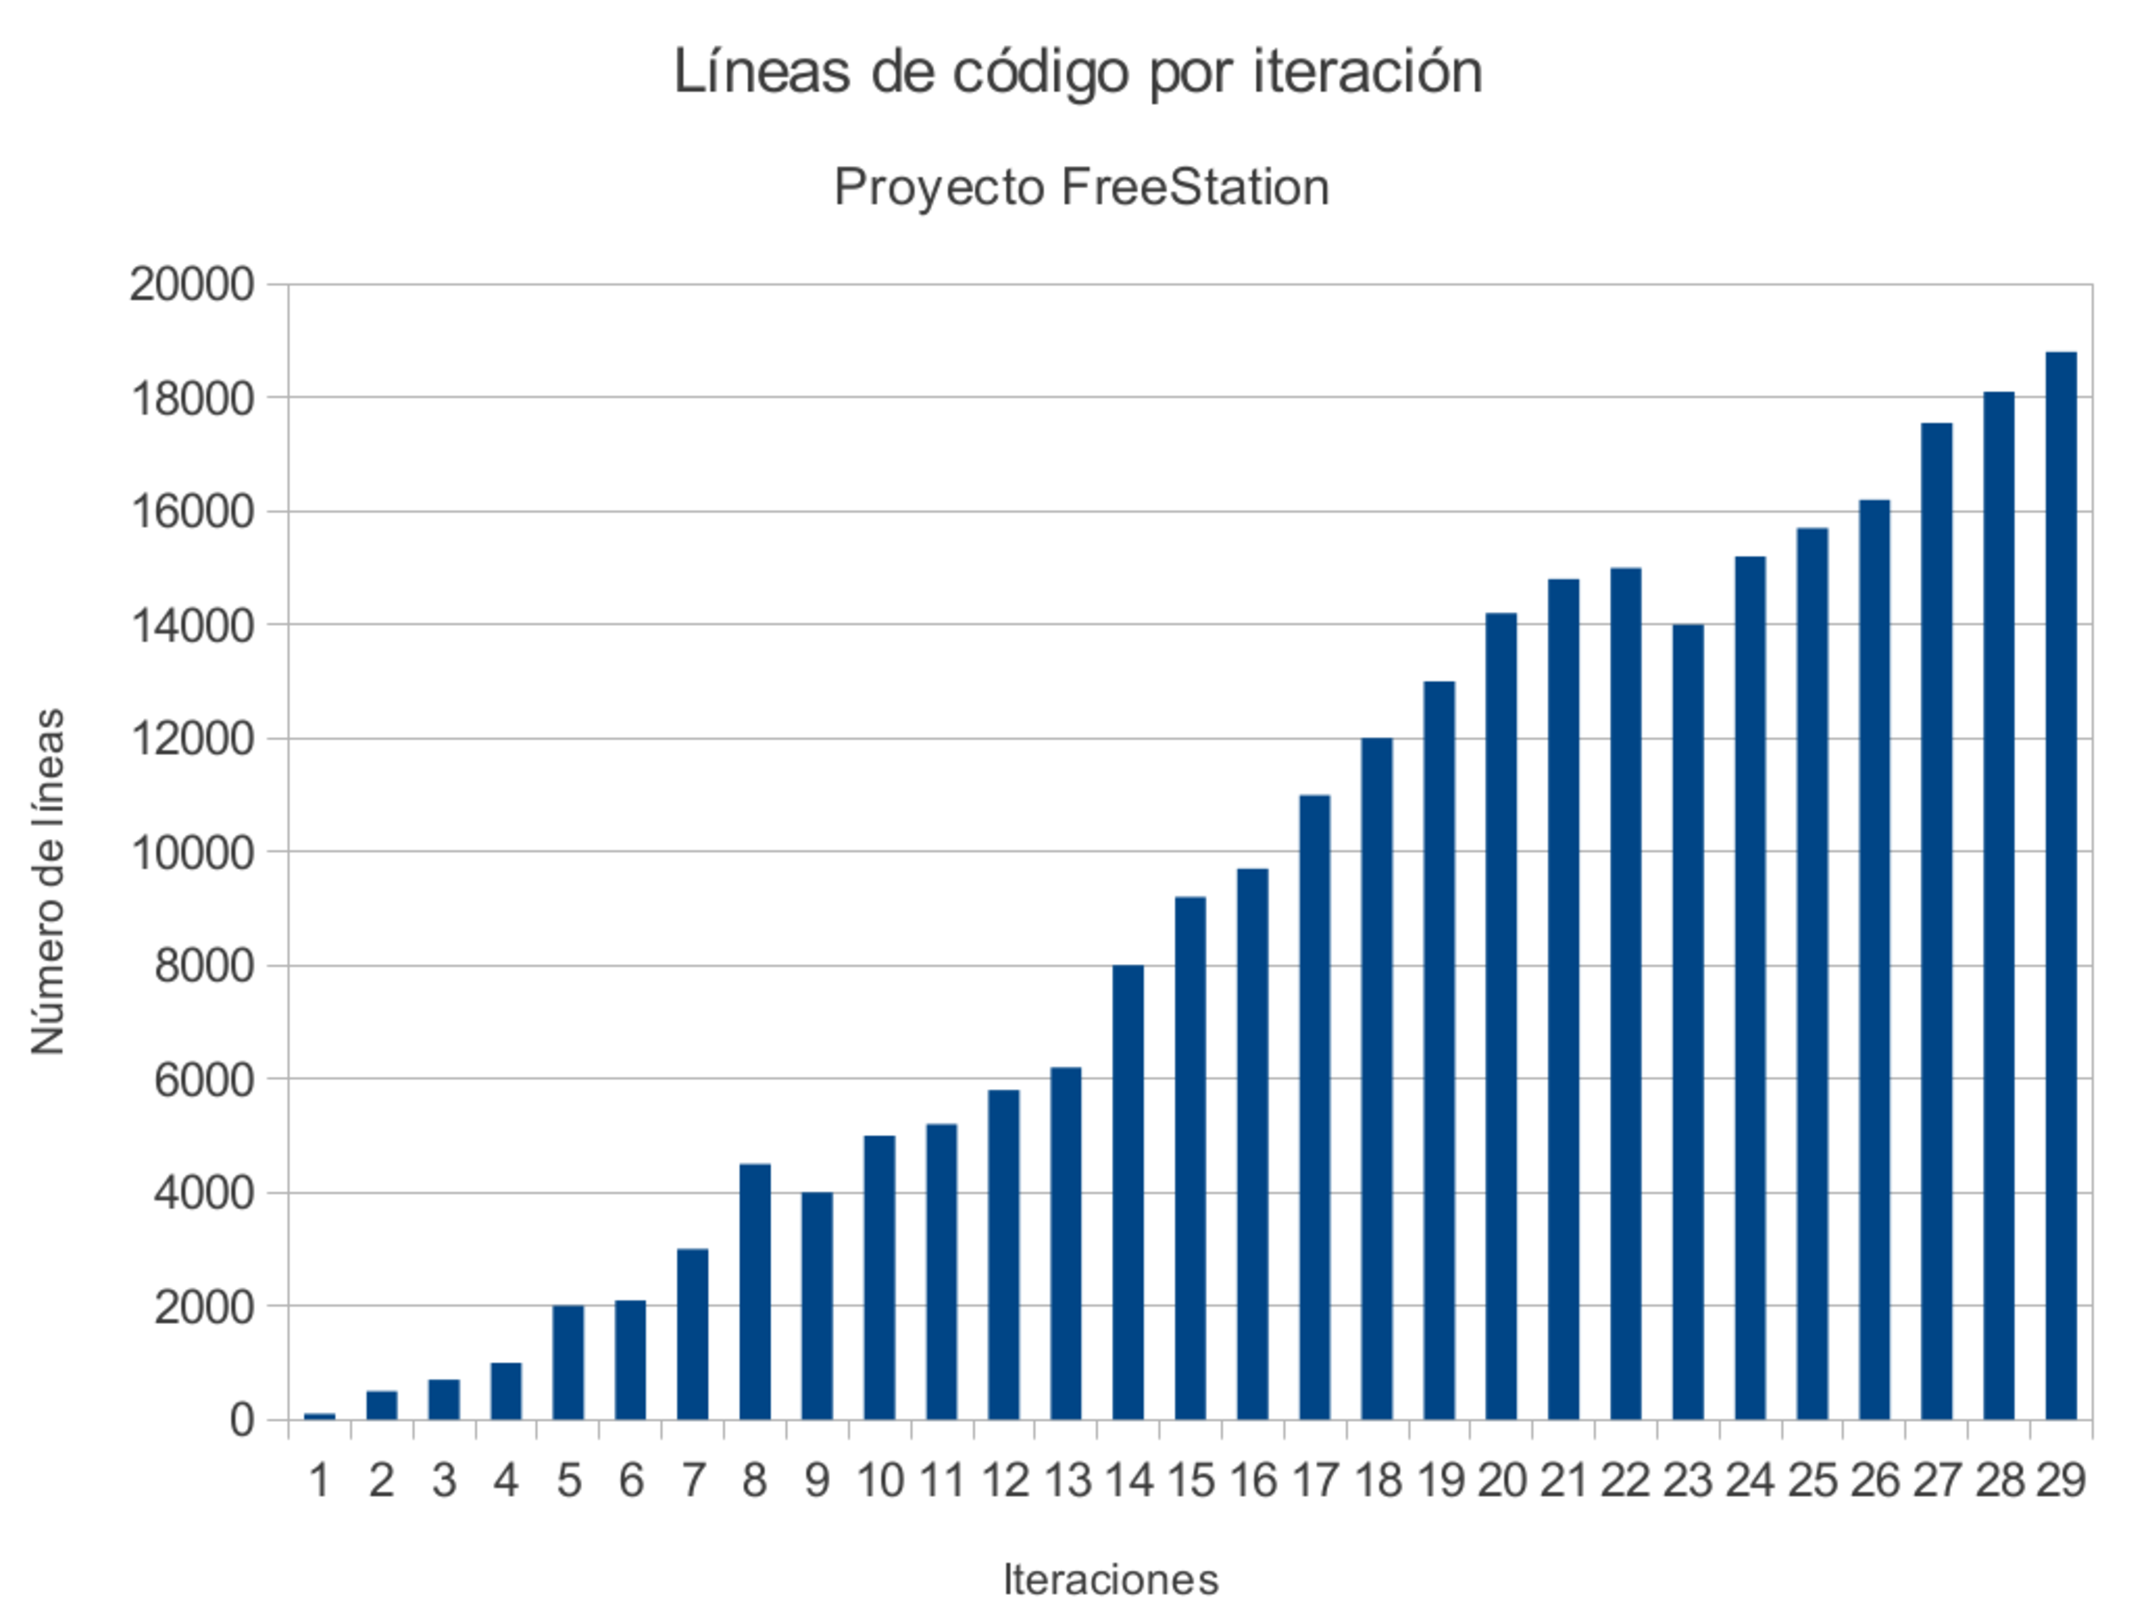
\includegraphics[width=425px]{src/img/diagrams/code-iteration.pdf}
        \caption[Líneas de código por iteración]
          {Líneas de código por iteración}
          \label{fig:codeiteration}
    \end{center}
\end{figure}

En la figura ~\ref{fig:codeiteration} se muestra un gráfico de la evolución de
las líneas de código fuente durante toda la etapa de desarrollo.

Se ha utilizado la herramienta cloc y sloccount para contabilizar las líneas de 
código fuente, asociado a los lenguajes en los que está programado
\emph{FreeStation}. Hay que tener en cuenta que dicha herramienta contabiliza
todas las líneas de código del proyecto, también las autogeneradas. 

\newpage

\textbf{Proyecto FreeStation web (Frontend y Backend Servidor)}

\begin{table}[ht]
    \centering
\begin{tabular}{|l|l|l|l|l|}
  \hline
  \multicolumn{5}{|c|}{Idiomas agrupados por lenguaje dominante primero}
  \\
  \hline
  Lenguaje & Archivos & Espacios en blanco & Comentarios & Líneas de código \\
  Javascript        &              19   &       2901      &     2177    & 10495\\ 
  HTML        &                    18        &    505   &     5     & 2797\\ 
  CSS          &                   14           & 507  &       141 & 2405\\ 
  PHP           &                  27         &   402   &     930  & 1999 \\
  Python       &                    8          &  367   &    348   &   876\\ 
  make         &                    1         &    24   &      5     &   124\\ 
  SQL        &                      2        &     37    &     57      &   82\\ 
  Bourne Shell  &                   2       &      22    &    6    & 48\\  
  XML           &                   1         &     0    &          0  &  10\\ 
  Total & 92    &       4765    &       3709       & 18836\\
  \hline
\end{tabular}
    \caption{Tabla líneas de código FreeStation web}
     \label{tab:slocweb}
\end{table}

Las estimaciones de SLOC son:

Development Effort Estimate, Person-Years (Person-Months) = 0.43 (5.19) \\
 (Basic COCOMO model, Person-Months = 2.4 * (KSLOC**1.05)) \\
Schedule Estimate, Years (Months)                         = 0.39 (4.67) \\
 (Basic COCOMO model, Months = 2.5 * (person-months**0.38)) \\
Estimated Average Number of Developers (Effort/Schedule)  = 1.11 \\
Total Estimated Cost to Develop                           = $ 58,410 \\
 (average salary = $56,286/year. \\

\textbf{Proyecto FreeStation client (Frontend y Backend cliente)}

\begin{table}[ht]
    \centering
\begin{tabular}{|l|l|l|l|l|}
  \hline
  \multicolumn{5}{|c|}{Idiomas agrupados por lenguaje dominante primero}
  \\
  \hline
  Lenguaje & Archivos & Espacios en blanco & Comentarios & Líneas de código \\
XML               &               7 &            44 &         30416 & 158519 \\
Python             &             79  &         1971  &         3584 & 4664 \\
Javascript          &             5   &         261   &         400 & 1249 \\
HTML                 &            2    &         16    &          1 & 141 \\
CSS                   &           2     &        27     &        13 & 123 \\
Bourne Shell           &          2      &        7      &        5 & 29 \\
Total                   &         97      &     2326      &    34419 & 164725 \\
  \hline
\end{tabular}
    \caption{Tabla líneas de código FreeStation client}
     \label{tab:slocclient}
\end{table}

\newpage

Las estimaciones de SLOC son:

Development Effort Estimate, Person-Years (Person-Months) = 41.46 (497.46) \\
 (Basic COCOMO model, Person-Months = 2.4 * (KSLOC**1.05)) \\
Schedule Estimate, Years (Months)                         = 2.21 (26.47) \\
 (Basic COCOMO model, Months = 2.5 * (person-months**0.38)) \\
Estimated Average Number of Developers (Effort/Schedule)  = 18.80 \\
Total Estimated Cost to Develop                           = $ 5,600,037 \\
 (average salary = $56,286/year, overhead = 2.40). \\

\section{\uppercase{Resultados}}

En esta sección se describen los resultados. Se muestran los
elementos más relevantes obtenidos al realizar pruebas con entornos reales.
También se realiza un estudio del rendimiento de la aplicación cuando a ésta 
se le conectan diferente número de clientes.

\subsection{Resultados con test unitarios}

Una comparación de los resultados obtenidos de los test unitarios son plenamente
satisfactorios. Todos los test pasan correctamente y han contribuido a
realizar un mejor desarrollo detectando fallos en la implementación. La batería
de pruebas no es completa pero si prueba las partes críticas de la aplicación.

\subsection{Profiling}

Profiling es como se conoce en ingeniería del software a la medida y 
análisis de rendimiento de una aplicación de forma dinámica, es decir, 
utilizando una ejecución concreta de dicha aplicación. El objetivo es determinar
qué partes del código son cuellos de botella (consumen más recursos), y por 
tanto, son más susceptibles de ser optimizadas.

En el profiling de \emph{FreeStation}, se ha utilizado el módulo de
python cProfile, herramienta libre para GNU/Linux.

Para realizar el análisis es necesario ejecutar el programa benchmark.py y este
ofrecerá los resultados al igual que otros test de rendimiento como el programa
benchmark\_microfiber.py para rendimiento en microfiber.

El profiler genera un documento a modo de informe del porcentaje de uso de CPU 
de cada una de las funciones individuales de la ejecución de la aplicación.
En la sección de arquitectura ~\ref{sec:classforcouchdb} se procedió a explicar
un análisis del mismo.